\documentclass[notheorems]{beamer}
\usepackage[utf8]{inputenc}
\usepackage{amsmath}
\usepackage{amsfonts}
\usepackage{amssymb}
\usepackage{polski}
\usepackage{amsmath}
\usepackage{centernot}
\usepackage{amsfonts}
\usepackage{amssymb}
\usepackage{amsthm}
\usepackage{enumerate}
\usepackage{mathtools}
\usepackage{hyperref}
\usepackage{algorithm,algorithmic}
\usepackage{natbib} %bibtex
\usepackage[polish]{dyschemist}
\newtheorem{tw}{Twierdzenie}
%\usepackage{dyschemist}
\author{Anna Szczepaniak, 210094}
\title{Algorytmy dekompozycji QR}
\date{19.09.2019}
\institute{Praca licencjacka przygotowana pod opieką dr, mgr inż. Piotra Kowalskiego}
\newcommand{\parauporzadkowana}[2]{\left\langle {#1}; {#2} \right\rangle}
\newcommand{\zbior}[1]{\left\lbrace {#1} \right\rbrace }
\newcommand{\domkniecie}[1]{\left[ {#1} \right] }
\newcommand{\notiff}{%
  \mathrel{{\ooalign{\hidewidth$\not\phantom{"}$\hidewidth\cr$\iff$}}}}
%\newcommand{\tuple}[1]{\left\langle {#1} \right\rangle}
\newcommand{\vr}[1]{\mathbf{#1}}
\newcommand{\mx}[1]{{#1}}
\newcommand{\sign}{\operatorname{sign}}
\newcommand{\proj}[2]{\frac{\scalar{#2}{#1}}{\scalar{#1}{#1}}}

\usepackage{Sweave}
\begin{document}
\begin{frame}
\titlepage
\end{frame}



\begin{frame}
\begin{theorem}[Nierówność Bessela {\citep[Twierdzenie 14.22]{poreda11}}] \label{Nierówność-Bessela}
Jeśli $(\vr{b}_{1}, \ldots, \vr{b}_{n})$ jest układem ortonormalnym w przestrzeni euklidesowej $\setR^k$, to dla każdego wektora $\vr{x}$ z przestrzeni $\setR^k$ spełniona jest nierówność 
$$
\sum_{i=1}^{n}\alpha_{i}^{2}\leq \Vert\vr{x}\Vert^{2},
$$
gdzie $\alpha_{i} = (\vr{x}|\vr{b}_{i})$. Ponadto, wektor $\vr{x} - \sum_{i=1}^{n} \alpha_{i} \cdot \vr{b}_{i}$ jest ortogonalny do podprzestrzeni $span(\vr{b}_{1}, \ldots, \vr{b}_{n})$.
\end{theorem}
\end{frame}

\begin{frame}
\begin{theorem}[Twierdzenie(Grama-Schmidta)\citep{poreda11}] \label{theorem-gram-schmidt}
Dla każdego układu liniowo niezależnego wektorów $(\vr{x}_{1},\ldots,\vr{x}_{n})$ w przestrzeni euklidesowej istnieje układ ortonormalny $(\vr{b}_{1},\ldots, \vr{b}_{n})$ taki, że 
$$
span(\vr{b}_{1},\ldots, \vr{b}_{k}) = span(\vr{x}_{1},\ldots, \vr{x}_{k})
$$
dla każdej liczby $k$ ze zbioru $(1,\ldots,n)$.
\end{theorem}
\end{frame}


\begin{frame}
\begin{theorem}[O rozkładzie QR]\label{theorem-qr-decomposition}
Niech $\mx{A} \in \setR^{m \times n}$, gdzie $m\ge n$, której kolumny są liniowo niezależne. Istnieje wtedy jedyny rozkład $\mx{QR}$, tzn. że istnieją takie macierze $\mx{Q}$ i $\mx{R}$, że
$$
\mx{A} = \mx{Q} \mx{R}
$$ 
i
\begin{itemize}
\item macierz $\mx{Q} \in \setR^{m \times n} $ jest taka, że 
$$
Q^{T}\cdot Q=D,
$$
gdzie $D= diag (d_{1}, d_{2}, ..., d_{n})$, oraz $d_{k}>0$ dla $k = 1, 2, \ldots, n$, oraz
\item macierz $\mx{R} \in \setR^{n \times n}$ jest trójkątną górną spełniającą dodatkowo warunek 
$$
r_{kk}= 1 
$$ 
dla wszystkich $k = 1, 2, \ldots, n$.
\end{itemize} 
\end{theorem}
\end{frame}

\begin{frame}
\begin{remark}
Rozkładem $\mx{QR}$ nazwiemy również sytuacje, gdy 
$$
\mx{A}=\mx{Q}\mx{R}
$$
oraz $\transpose{\mx{Q}}\mx{Q}=\mx{I}$ i $\mx{R}$ jest macierzą trójkątną górną, niekoniecznie z $1$ na przekątnej. Powodem tego jest, że prezentowana tu postać oraz postać z twierdzenia \ref{theorem-qr-decomposition} są sobie równoważne.  
\end{remark}
\end{frame}


\begin{frame}
\begin{definition}[Macierz Householdera]
Macierzą Householdera $H$, zwaną również refleksją, nazywamy macierz postaci 
$$
\mx{H}=\mx{I}-2\cdot \vr{v}\cdot \vr{v}^{T},
$$
gdzie $\Vert v \Vert_{2} = 1$.
\end{definition}
\end{frame}

\begin{frame}
\begin{theorem} [Transformacja Householdera]
Niech  $\vr{v}\in R^{m}, $ i $\vr{v}\neq 0. $ Wówczas transformacją Householdera nazywamy macierz postaci:
$$
\mx{H}=\mx{I}-W\vr{v}\vr{v}^{T},
$$
gdzie
$$
W={\frac {2}{\vr{v}^{T}\vr{v}}}.
$$ 
Macierz H jest macierzą symetryczną i ortogonalną.
\end{theorem}
\end{frame}

\begin{frame}
\begin{definition}[Macierz Givensa]
Niech $ i,j \in {1, \ldots, n}$ i $\theta \in \setR$. Macierz $\mx{R}(i,j,\theta) \in \setR^{n\times n}$ zdefiniowana następująco:
$$
\mx{R}(i,j,\theta) = \begin{bmatrix}
1       & 0     & \cdots &    0       & \cdots &    0       & \cdots & 0 & 0& \\
0       & 1     & \cdots &     0      & \cdots &     0      &  \cdots& 0 & 0 &   \\
0       & 0     & \ddots &     0      &  \cdots&     0      &  \cdots& 0 & 0 &  \\
\vdots  &\vdots &  \cdots& \cos\theta & \cdots & -\sin\theta&  \cdots& 0 & 0& \\
0       &  0    & \cdots & \vdots     &  \ddots&  \vdots    & \cdots & 0 & 0& \\
\vdots  & \vdots& \cdots & \sin\theta & \cdots & \cos\theta &  \cdots& 0 & 0& \\
0       & 0     & \cdots &    0       &  \cdots&  0         & \ddots &  0& 0& \\
\vdots  & \vdots&\cdots  &  \cdots    &  \cdots&  \cdots    & \cdots & 1 & 0&\\
0       & 0     & \cdots &     0      &  \cdots&    0       &  \cdots& 0 & 1 & \\       
\end{bmatrix}
$$
nazywamy macierzą rotacji Givensa.
\end{definition}
\end{frame}

\begin{frame}[fragile]
\begin{Schunk}
\begin{Sinput}
> house = function(x) {
+   norm_x = sqrt(t(x)\cdot x)
+   if (x[1] > 0) {
+     x[1] = x[1] + norm_x;
+   } else {
+     x[1] = x[1] - norm_x;
+   }
+   return(x)
+ }
\end{Sinput}
\end{Schunk}
\end{frame}


\begin{frame}[fragile]
\begin{Schunk}
\begin{Sinput}
> qr_householer = function(A)
+ {
+  R = A
+  dimm = dim(A)
+  n = dimm[2]
+   m = dimm[1]
+   Q = diag(n)
+   for (i in 1:min(m-1,n)){
+     u = house(R[i:m,i])
+     den =  (t(u) %*% u)[1,1]
+     P = diag(n+1-i) - 2/den * ( u%*% t(u)  ) 
+     R[i:m,i:n] = P %*% R[i:m,i:n]
+     if (i>1)
+       Q[i:n,1:(i-1)] = P %*% Q[i:n,1:(i-1)]
+     Q[i:n,i:n] = P %*% Q[i:n,i:n]
+   }
+   return(list(R=R, Q=t(Q)))
+ }
\end{Sinput}
\end{Schunk}
\end{frame}



\begin{frame}[fragile]
\begin{Schunk}
\begin{Sinput}
> givens = function(i,j,A){
+   dimm = dim(A)
+   n = dimm[1]
+   G = diag(n)
+   p = sqrt((A[i,i])^2 + (A[j,i])^2)
+   G[i,i] = A[i,i]/ p
+   G[i,j] = (A[j,i])/p
+   G[j,i] = -(A[j,i])/p
+   G[j,j] = A[i,i]/ p
+   
+ return(G)  
+   
+ }
\end{Sinput}
\end{Schunk}
\end{frame}

\begin{frame}[fragile]
\begin{Schunk}
\begin{Sinput}
> qr_givens = function(A){
+   R = A
+   
+   n = dim(A)[2]
+   m = dim(A)[1]
+   Q = diag(n)
+   for (i in 1:(n-1)) {
+     for (j in (i+1):m) {
+       G = givens(i,j,R)
+       R = G %*% R
+       Q = Q %*% t(G)
+     }
+   }
+   return(list(R=R, Q=Q))
+ }
\end{Sinput}
\end{Schunk}
\end{frame}


\begin{frame}
Rozmiar macierzy nie wpływa istotnie na jakość naszych samodzielnie opisanych funkcji w stosunku do gotowej funkcji w R. Są one mniej dokładne niż wbudowany, gotowy algorytm dekompozycji QR w R. Ponadto algorytm metodą rotacji Givensa nie zawsze jest jakościowo lepszy od algorytmu metodą odbić Householdera. Zależy to od wymiarów oraz od losowości rozkładanej macierzy.
\end{frame}

\begin{frame}[fragile]
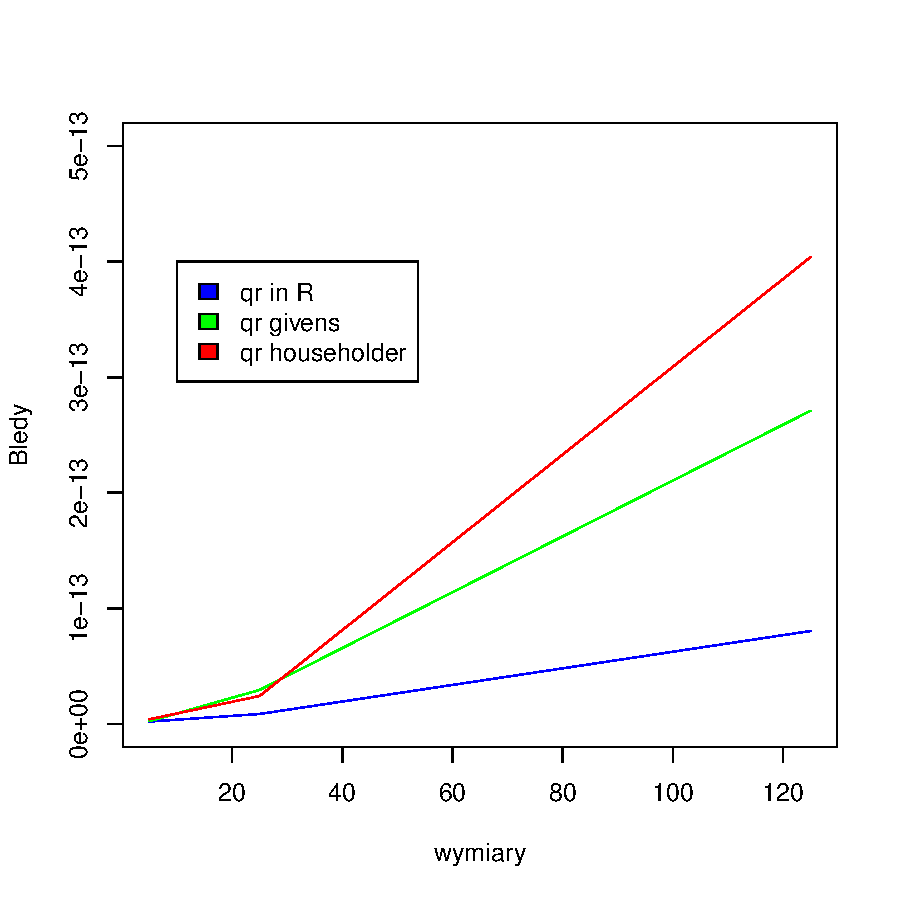
\includegraphics{licencjat-027}
\end{frame}

\end{document}